%%____________________________________________________________________________||
\section{Search sensitivity}
\label{sec:sensitivity}
\subsection{Likelihood model}

Consider a given category of event as defined by \njet and \nb.

%%%%%%%%%%%%%%%%%%%%%%%%%%%%%%%%
\subsubsection{Hadronic sample}
\label{sec:hadronicLikelihood}
%%%NOTE - MUST CHANGE SYSTEMATICS WHEN DECIDED HOW TO PROPERLEY DEAL WITH THEM!!!!!
Let $N$ be the number of bins of \HT, which need not have equal width.
Let $n^i$ represent the number of events observed satisfying all
selection requirements in each \HT bin $i$.  Then the likelihood of
the observations is written this way:

\begin{equation}
L_{hadronic}=\prod_i \mathrm{Pois}(n^i |\, b^i + s^i)
\label{eq:hadronicLikelihood}
\end{equation}

where $b^i$ represents the expected Standard Model background in bin
$i$, $s^i$ represents the expected number of signal events in bin $i$,
and $\mathrm{Pois}$ represents the Poisson distribution.  It is
assumed that:

\begin{equation}
  b^i\equiv \ewk^i
  \label{eq:ewkTotal}
\end{equation}

where $\ewk^i$ is the expected yield of electroweak events in bin $i$.
By construction, the contribution from QCD events is expected to be negligible, 
Sec.~\ref{sec:qcd}



%%%%%%%%%%%%%%%%%%%%%%%%%%%%%%%%
\subsubsection{Electroweak control samples\label{sec:ewk}}

Let \fZinv{i} represent the expected yield from \znunu in bin $i$
divided by the expected electroweak background $\ewk^{i}$.  It is
a floating parameter limited between zero and one.

Let:

\begin{equation}
  \zInv{i} \equiv \fZinv{i} \times \ewk^i 
  \label{eq:ZinvEwk}
\end{equation}

\begin{equation}
  ttW^{i} \equiv (1-\fZinv{i})\times \ewk^i
  \label{eq:ttWEwk}
\end{equation}

The variable $\zInv{i}$ thus represents the expected number of \znunu
events in \HT bin $i$ of the hadronically selected sample, and the
variable $ttW^i$ represents the expected number of events from SM
$W$-boson production (including top quark decays) in \HT bin $i$ of
the hadronically selected sample.

In each bin $i$ of \HT, there are three measurements: $n_{ph}^i$,
$n_{\mu}^i$, and $n_{\mu\mu}^i$, representing the event counts in the
photon, single-muon, and double-muon control samples.  Each of these
measurements has a corresponding yield in simulated data: $MC_{ph}^i$,
$MC_{\mu}^i$, and $MC_{\mu\mu}^i$.  The simulation also gives expected
amounts of $\zInv{}$ and $t\bar{t}+W$ in the hadronically-selected
sample: $MC_{\zInv{}}^i$ and $MC_{t\bar{t}+W}^i$.  After defining

\begin{equation}
r_{ph}^i = \frac{MC_{ph}^i}{MC_{\zInv{}}^i};\, r_{\mu\mu}^i =
\frac{MC_{\mu\mu}^i}{MC_{\zInv{}}^i};\, r_{\mu}^i =
\frac{MC_{\mu}^i}{MC_{t\bar{t}+W}^i}\quad ,
\end{equation}

these likelihood functions are used:

\begin{equation}
\label{eq:photonLikelihood}
L_{ph}= \prod_i \mathrm{Pois}(n_{ph}^i |\, \rho_{phZ}^j \cdot
r_{ph}^{i} \cdot \zInv{i})
\end{equation}

\begin{equation}
\label{eq:mumuLikelihood}
L_{\mu\mu}=\prod_i \mathrm{Pois}(n_{\mu\mu}^i |\, \rho_{\mu\mu Z}^j
\cdot r_{\mu\mu}^{i} \cdot \zInv{i})
\end{equation}

\begin{equation}
\label{eq:muonLikelihood}
L_{\mu}=\prod_i \mathrm{Pois}(n_{\mu}^i |\, \rho_{\mu W}^j \cdot
r_{\mu}^{i} \cdot ttW^{i} + s_{\mu}^i)\quad .
\end{equation}

Equation~\ref{eq:photonLikelihood} can be used to estimate the maximum
likelihood value for $\zInv{i}$ (the expectation for the \znunu\ +
jets background in the hadronic signal region) given the observations
$n_{ph}^i$ in the photon control sample and the ratios $r_{ph}^i$. A
similar construction is used when estimating $\zInv{i}$ from the
di-muon control sample (Equ.~\ref{eq:mumuLikelihood}) and $ttW^{i}$
from the single muon control sample
(Equ.~\ref{eq:muonLikelihood}). The measurements in each of the
control samples and the hadronic signal region, along with the ratios
$r_{ph}^{i}$, $r_{\mu\mu}^{i}$, and $r_{\mu}^{i}$, are all considered
simultaneously through the relationships defined in
Equs.~\ref{eq:ewkTotal}, \ref{eq:ZinvEwk}, and
\ref{eq:ttWEwk}. The ratios $r_{ph}^{i}$, $r_{\mu\mu}^{i}$, and
$r_{\mu}^{i}$ are simply the inverse of the translation factor (1/TF)
defined in Equ.~\ref{equ:pred-method}
(Sec.~\ref{sec:background-method}). More specifically, $MC_{ph}^i$,
$MC_{\mu}^i$, and $MC_{\mu\mu}^i$ are the yields obtained from MC
after applying the selection criteria for the photon, single muon and
di-muon samples, as defined by Equ.~\ref{equ:ratio-denom}
(Sec.~\ref{sec:background-method}). The variables $MC_{t\bar{t}+W}^i$ and
$MC_{\zInv{}}^i$ are defined by Equs.~\ref{equ:ratio-numer-mj} and
\ref{equ:ratio-numer-mmj} (Sec.~\ref{sec:background-method}), respectively.

The parameters $\rho_{phZ}^j$, $\rho_{\mu\mu Z}^j$, and $\rho_{\mu
  W}^j$ represent ``correction factors'' that accommodate the
systematic uncertainties associated with the control-sample-based
background constraints.  The quantities $\sigma_{phZ}^j$,
$\sigma_{\mu\mu Z}^j$, and $\sigma_{\mu W}^j$ represent the relative
systematic uncertainties for the control sample constraints, taken
into account with the following terms:

\begin{equation}
\label{eq:ewkSyst}
L_{\rm EWK\, syst.}=\prod_j \mathrm{Logn}( 1.0 |\,\rho_{\mu W}^j,
\sigma_{\mu W}^j)\times \mathrm{Logn}( 1.0 |\,\rho_{\mu\mu Z}^j,
\sigma_{\mu\mu Z}^j)\times \mathrm{Logn}( 1.0 |\,\rho_{phZ}^j,
\sigma_{phZ}^j) \quad ,
\end{equation}

where Logn is the log-normal
distribution~\cite{cousins-log-normal}:

\begin{equation}
\label{eq:log-normal}
\mathrm{Logn}(x |\,\mu,\sigma_{\mathrm{rel.}}) =
\frac{1}{x\sqrt{2\pi}\ln{k}}\exp{\left(-\frac{\ln^2{\left(\frac{x}{\mu}\right)}}{2\ln^2{k}}\right)};\quad
k=1+\sigma_{\mathrm rel.}\quad. 
\end{equation}

Seven (resp. one) parameters per control sample are used to span up to
eleven (resp. four) \HT bins, as shown in Table~\ref{tab:systMap}.

\begin{table}\centering
\caption{The systematic parameters used in \HT bins.  Left: categories
  with up to eleven bins; right: category with four bins.}
\label{tab:systMap}
\footnotesize
\begin{tabular}{lccccccccccc}
\hline
\hline
\HT bin ($i$)         & 0 & 1 & 2 & 3 & 4 & 5 & 6 & 7 & 8 & 9 & 10 \\
\hline
syst. parameter ($j$) & 0 & 1 & 2 & 3 & 3 & 4 & 4 & 5 & 5 & 6 & 6 \\
\hline
\hline
\end{tabular} \ \ 
\begin{tabular}{lccccc}
\hline
\hline
\HT bin ($i$)         & 0 & 1 & 2 & 3\\
\hline
syst. parameter ($j$) & 0 & 0 & 0 & 0\\
\hline
\hline
\end{tabular}
\end{table}

\newcommand{\rpi}{\ensuremath{r_{\mu}^{\prime\ i}}\xspace}

Alternatively, the single muon sample can be used to constrain the
total EWK background thus:

\begin{equation}
\rpi \equiv \frac{MC_{\mu}^i}{MC_{t\bar{t}+W+\zInv{}}^i}\quad ;
\end{equation}
\begin{equation}
\label{eq:muonLikelihoodTotalEwk}
L_{\mu}=\prod_i \mathrm{Pois}(n_{\mu}^i |\, \rho_{\mu W}^j \cdot
\rpi \cdot \ewk^{i} + s_{\mu}^i)\quad .
\end{equation}

The photon and di-muon likelihoods are dropped, as are the parameters
\fZinv{}.

%%%%%%%%%%%%%%%%%%%%%%%%%%%%%%%%
\subsubsection{Contributions from signal}
\label{sec:signalContrib}

Let $x$ represent the cross section for a particular signal model, and
let $l$ represent the recorded luminosity.  Let $\epsilon^{i}_{had}$
(resp.  $\epsilon^{i}_{\mu}$) be the analysis efficiency as simulated
for the model in \HT bin $i$ of the hadronic (resp. single muon
control) sample.  Let $\delta$ represent the relative uncertainty on
the signal yield, assumed to be fully correlated among the bins, and
let $\rho_{sig}$ represent the ``correction factor'' to the signal
yield which accommodates this uncertainty.  Let $f$ represent an
unknown multiplicative factor on the signal cross section, for which
an allowed interval shall be determined.

Then the expected hadronic signal yield $s^i$ from
Equation~\ref{eq:hadronicLikelihood} is written as $s^i \equiv
f\rho_{sig} xl\epsilon_{had}^i$, and the ``signal contamination'' in
the muon control sample $s_{\mu}^i$ from
Equation~\ref{eq:muonLikelihood} is treated analogously: $s_{\mu}^i
\equiv f\rho_{sig} xl\epsilon_{\mu}^i$.  The systematic uncertainty on
the signal efficiency is included via an additional term in the
likelihood:

\begin{equation}
L_{sig}=\mathrm{Logn}(1.0 |\,\rho_{sig}, \delta) \quad .
\end{equation}

%%%%%%%%%%%%%%%%%%%%%%%%%%%%%%%%
\subsubsection{Total likelihood}
\label{sec:totalLikelihood}

The likelihood function for a given selection $k$ is the product of
the terms described in the previous sections:

\begin{equation}
L^k = L_{hadronic}^k \times L_{\mu}^k \times L_{ph}^k \times
L_{\mu\mu}^k\times L_{\rm EWK\, syst.}^k \quad .
\end{equation}

In a category with 11 \HT bins and three control samples (single muon,
di-muon, and photon), there are 40 nuisance parameters:
$\{\ewk^{i}\}_{i=0}^{10}$, $\{\fZinv{i}\}_{i=0}^{10}$, $\rho_{phZ}^j$
(with $j=3,4,5,6$), $\rho_{\mu\mu Z}^j$, $\rho_{\mu W}^j$, (with
$j=0,1,2,3,4,5,6$).  In a category with eight \HT bins and one control
sample (single muon), there are 18 nuisance parameters (drop
$\{\fZinv{i}\}_{i=0}^{10}$, $\rho_{phZ}^j$, $\rho_{\mu\mu Z}^j$).  In
a category with three \HT bins and one control sample (single muon),
there are five nuisance parameters: $\ewk^{0,1,2,3}$, $\rho_{\mu
  W}^0$.  When considering signal, there is also the parameter
$\rho_{sig}$; when multiple categories are fit simultaneously, the
total likelihood is


\begin{equation}
L = L_{sig}\times \prod_k L_{hadronic}^k
\times L_{\mu}^k \times L_{ph}^k \times L_{\mu\mu}^k \times L_{\rm EWK\, syst.}^k \quad .
\end{equation}

\subsection{Signal models and efficiencies\label{sec:signal}}
To interpret the results of this search, simplified
models~\cite{Alwall:2008ag,Alwall:2008va,sms} are used. These
effective models use only a limited set of sparticles (production and
decay) and enable comprehensive studies of individual SUSY event
topologies. The simplified model studies can be performed in terms of
fundamental properties such as decay modes, production cross sections,
and sparticle masses. As gluinos provide an early discovery potential, the model
T1bbbb is used here to demonstrate sensitivity.

Signal efficiency times acceptance is determined per model per event
category (\njet,\nb) per \scalht bin. Systematic
uncertainties on the signal efficiencies are determined per model
following the 2012 analysis (see Section~\ref{sec:sms-syst}). Due to CPU
limitations, only a subset of event categories (but all \scalht bins
within a category) are considered for interpretation with each
simplified model. 

%The efficiency time acceptance for an inclusive

%selection on \scalht and for the relevant categories are shown.
The simplified models considered for the Phys14 exercise are summarised in
Table~\ref{tab:simplified-models}. The event categories considered for
each model interpretation are listed. The choice of which categories
is made by comparing the expected upper limit on the signal cross section 
per model mass point achieved for each individual event category. 
The categories are then ranked according to their expected (exclusion) reach 
and the most sensitive categories are used. 

%The second method is based on a signal
%injection test that highlights the expected signal significance per
%signal region bin. The event categories that demonstrate the largest
%significances across all \scalht bins are chosen. The former method is
%presently used.

\begin{table}[h!]
  \caption{A summary of the simplified models considered for
    interpretation. The event categories considered for each model are
    listed.}  
  \label{tab:simplified-models}
  \setlength{\extrarowheight}{2.5pt}
  \centering
  \begin{tabular}{ llcc }
    \hline
    \hline
    Model                   & Production/decay mode & (\njet,\nb) event categories considered        \\ 
    \hline
    \texttt{T1bbbb}           & \Tonebbbb               & (4,2),(4,3),(4,4),($\geq 5$,2), ($\geq 5$,3),($\geq 5$,$\geq 4$) \\ % (2--3,1), 
    % \texttt{T2bw (x=0.25)}  & \Ttwobw               & FIXME: ANA-CATS \\
    % \texttt{T2bw (x=0.75)}  & \Ttwobw               & FIXME: ANA-CATS \\
    % \texttt{T2tt}           & \Ttwott               & FIXME: ANA-CATS \\
    \hline
    \hline
  \end{tabular}
\end{table}
\subsection{Efficiency times acceptance for \texttt{T1bbbb}\label{sec:t1bbbb-eff}}

Table ~\ref{tab:simplified-models} shows the
expected signal efficiency times acceptance for the signal region and
\mj control sample (\ie, signal contamination) for the model
\texttt{T1bbbb} in the four most sensitive (\njet,\nb) event categories.
An inclusive selection on \scalht ($>200\gev$) is used. 
[CHOOSE ME]. 

\begin{table}[h!]
  \caption{A summary of the simplified models considered for
    interpretation. The event categories considered for each model are
    listed.}  
  \label{tab:simplified-models}
  \setlength{\extrarowheight}{2.5pt}
  \centering
  \begin{tabular}{ llcc }
    \hline
    \hline
    Category    & Efficiency times acceptance\\
    \hline
    (4,2)	& $0\%$	\\
    (4,3)	& $0\%$	\\
    (4,4)	& $0\%$	\\
    ($\geq 5$,2)& $0\%$	\\
    ($\geq 5$,3)& $0\%$	\\
    ($\geq 5$,$\geq 4$)	&$0\%$	\\ % (2--3,1), 
    \hline
    \hline
  \end{tabular}
\end{table}

The efficiencies are typically around $5\%$ ($~25\%$ total). Get final results on this soon.
Suggests we will be able to make a very good limit.
The signal efficiency in the \mj control sample is
negligible with respect to the signal region. By extension, the
relative contamination for the \mmj sample is also considered to be
negligible. Regardless, any potential contamination is accounted for
in the likelihood model.

\subsection{Systematic uncertainties on signal efficiency times}


For the Phys14 exercise the systematic uncertainty for the signal region 
is assumed to be unchanged from that in the previous analysis. 
Thus a systematic uncertainty of $15\%$ is applied. The systematic 
uncertainty in the signal acceptance times efficiency is determined per mass 
point per event category (\njet,\nb) per
\scalht bin (inclusive on $\scalht > 200$). The effect of
uncertainties on the luminosity measurement, the parton distribution
functions, the jet energy scale, initial state radiation, and the
efficiencies of various cuts (including the \mht/\met filter, the
``dead ECAL'' filter, etc)
%and the lepton/photon vetoes)
used in the candidate signal event selection are considered. Each
contribution is considered to be independent and all contributions are
summed in quadrature to obtain a total systematic uncertainty per mass
point per category per \scalht bin. 

\subsection{Results}


\begin{figure}[h!]
  \begin{center}
      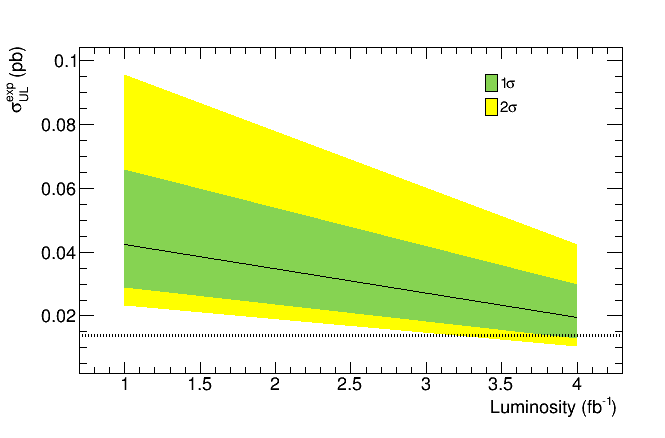
\includegraphics[width=0.8\textwidth]{figures/limit} % lbrt
      %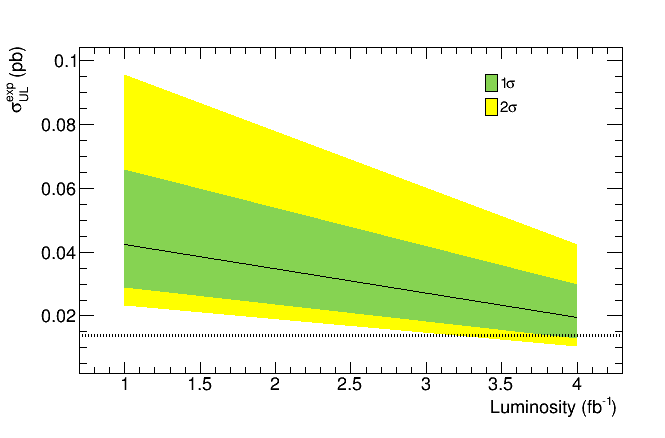
\includegraphics[width=0.45\textwidth, trim=0 190 290 20, clip=true ]{figures/limit} % lbrt
  \end{center}
 \caption{Limit at 1 and 4 fb for \texttt{T1bbbb}}
     \label{fig:limit}
\end{figure}
Assuming a systematic uncertainty of $0.15$ on the signal and taking the systematic
uncertainties on the backgrounds as $0.10$ (\scalht 200-600), $0.20$ (\scalht 600-1000),
$0.30$ (1000-$\inf$). The \scalht bins used were motivated as detailed in ???. Using the 
likelihood model from \ref{sec:hadronicLikelihood} and the \mj control sample (as $\nb > 1$) 
a limit was found for the \texttt{T1bbbb} model for luminosities of 1 and 4 fb. This is shown along 
with the theoretical cross section in \ref{fig:limit}. At 4fb it can be seen that we exclude to 1 million sigma.



%Comment to let me make a commit called first draft



%%____________________________________________________________________________||
